

\documentclass[accentcolor=tud4c,9.5pt,nochapname,bigchapter,paper=a5report]{tudreport}


\usepackage{mathtools}
\usepackage[pdftex,bookmarks=true]{hyperref}

\usepackage{lscape}
\usepackage{hyperref}
\usepackage{graphicx}
\usepackage{trfsigns}


\DeclareMathSizes{9.5}{9.5}{7}{7}
\DeclareMathSizes{10}{10}{7}{7}
\DeclareMathSizes{11}{11}{8}{8}

\usepackage{array}
\newcolumntype{+}{>{\global\let\currentrowstyle\relax}}
\newcolumntype{^}{>{\currentrowstyle}}
\newcommand{\rowstyle}[1]{\gdef\currentrowstyle{#1}%
#1\ignorespaces
}
\begin{document}

\def\Var{{\rm Var}\,}
\def\E{{\rm E}\,}
\def\freq{{\left(e^{j\omega}\right)}\,}


\title{Digital Signal Processing}
\subtitle{Formulary}
\subsubtitle{Author: Daniel Thiem - studium@daniel-thiem.de\\Version 0.7.3 - 17.02.2013}

\maketitle
\newpage
\thispagestyle{plain}
\mbox{}
\tableofcontents


\numberwithin{equation}{chapter}
\section*{Preface}
This formulary is based on the formulary of the course Stochastic Signals and Systems,
 which can be found here \url{https://github.com/Tyde/stosigsysfs/blob/master/document.pdf?raw=true}.
If you find any errors or have any ideas for improvement, mail me at studium@daniel-thiem.de
 or file an issue at \url{https://github.com/Tyde/dspformulary/issues}. The \LaTeX{}  source code is
online on \url{https://github.com/Tyde/dspformulary} and can be improved and extended.

\chapter{Digital Processing of Continous-Time Signals}
\section{Periodic Sampling}
Basic principles of sampling and transforming signals can be found in the Stochastic Signals and Systems formulary
\subsection{Reconstruction of Band-Limited Signals}
Assume, that $H_r(j\Omega)$ and $h_r(t)$ are the frequency and time responses for an ideal low pass filter where 
$x(n)$ is the input signal. Then the output will be
\begin{equation}
	x_r(t) = \sum\limits_{n=-\infty}^{\infty} x(n)h_r(t-nT)
\end{equation}
Because the filter is assumed to be ideal, its impulse response is given by:
\begin{equation}
	h_r(t)=\frac{\sin(\pi t/T)}{\pi t/T}
\end{equation}
where T is the sampling interval that should fulfil the Nyquist condition $\Omega_s > 2 \Omega_B$\\
Rules and correspondences can be found on the last page of the DSP-Script
\subsection{Discrete-time Processing of Continous-Time Signals}
To process a continous-time signal $x_c(t)$ with digital signal processing techniques, the following setup is used:\\
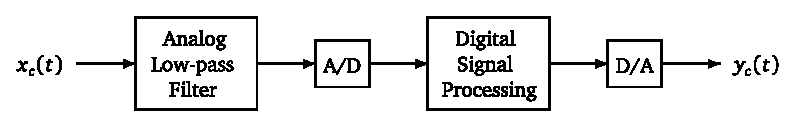
\includegraphics[width=\textwidth]{figures/dsp_setup.pdf}

\chapter{Digital Filter Design}

Let $x(n)$ and $y(n) , n=0\pm 1,\ldots$ be the input and the output of the system.  
Linear time-invariant discrete-time systems can be characterized 
 by linear constant coefficient difference equations of the following type, where $\max(N-1,M)$ is the order:
 \begin {equation}
 \sum\limits_{k=0}^{M}a_ky(n-k)= \sum\limits_{r=0}^{N-1} b_r x(n-r)
 \end{equation}
\section{Finite Impulse Response (FIR) filter}
If $M=0$ then the impulse response of the filter is finite so that:
\begin{subequations}
\begin{align}
y(n) &= \frac{1}{a_0}\sum\limits_{k=-\infty}^{\infty}b_r x(n-k) \\
\text{comparison with } &\text{the convolution sum yields} \notag \\
h(n) &= \begin{cases}
b_n/a_n, &n=0,\ldots,N-1\\
0, &\text{otherwise}
\end{cases}
\end{align}
\end{subequations}
\subsection{Properties of Filters}
With $f_{SR}$ being the sample rate.
The filter order has to fit to the requirement of the filter type for N (odd or even)
\begin{align}
\text{Filter Order}&=N-1
\Delta\omega &= \frac{f_s-f_p}{f_{SR}} 2\pi\\
\text{Delay} &=\frac{N-1}{2}
\end{align}

\section{Linear Phase Filters}
A digital filter can be described as linear phase filter if $H\freq$ can be expressed as:
\begin{equation}
	H\freq = H_M\freq e^{-j\omega \alpha}
\end{equation} 
with $H_M\freq$ real and $\alpha$(group delay) constant 

\subsection{Generalized linear phase system} \label{genLPS}
A Linear phase system with:
\begin{equation}
	H\freq = H_M\freq e^{-j\omega \alpha + j\beta}
\end{equation}
has to meet the condition:
\begin{equation} 
	\sum\limits_{n=-\infty}^{\infty} h(n)\sin[\omega (n-\alpha )+\beta] = 0 \forall \omega \in \mathbb{R}
\end{equation}

\section {Linear Phase FIR filters}
Applying the condition for generalized linear phase systems (\ref{genLPS}) to the FIR Filters yields two possible causal FIR Systems:
\begin{subequations}
\begin{align}
h(n) &= \begin{cases}
h(N-1-n)	&,0\leq n \leq N-1 \\
0			&,\text{otherwise} 
\end{cases} \\
H\freq &= H_e\freq e^{-j\omega (N-1)/2}
\end{align}
\end{subequations}
{\center and}
\begin{subequations}
\begin{align}
h(n) &= \begin{cases}
-h(N-1-n)	&,0\leq n \leq N-1 \\
0			&,\text{otherwise} 
\end{cases} \\
H\freq &= H_o\freq e^{-j\omega (N-1)/2+j\pi /2}
\end{align}
\end{subequations}

\section {Linear Phase FIR filter Types}
The linear phase FIR filters have been classified into 4 Types:

\begin{itemize}
  \item {\bf Type I} \quad symmetric impulse response and N is odd
  \item {\bf Type II}\quad symmetric impulse response and N is even
  \item {\bf Type III}\quad antisymmetric impulse response and N is odd
  \item {\bf Type IV}\quad antisymmetric impulse response and N is even
\end{itemize}

\subsection {Type I FIR linear phase filter}
$N$ is odd and the impuls response is symmetric. $\beta=0$ 
\begin{subequations}
\begin{align}
	h(n)&=h(N-1-n) \quad 0\leq n \leq N-1 \\
	H\freq &= e^{-j\omega \frac{N-1}{2}}\left[{\sum\limits_{k=0}^{(N-1)/2} a(k)\cos(\omega k)}\right]\\
	&\quad\text{where}\notag\\
	a(0)=h\left(\frac{N-1}{2}\right) \text{ and } a(k)&=2h\left(\frac{N-1}{2}-k\right), \quad\quad k=1,2,\ldots,(N-1)/2 \notag
\end{align}
\end{subequations}

\subsection {Type II FIR linear phase filter}
$N$ is even and the impuls response is symmetric. $\beta=0$ 
\begin{subequations}
\begin{align}
	h(n)&=h(N-1-n) \quad 0\leq n \leq N-1 \\
	H\freq &= e^{-j\omega \frac{N-1}{2}}\left\{{\sum\limits_{k=1}^{N/2} b(k)\cos\left[\omega \left(k-\frac{1}{2}\right)\right]}\right\}\\
	&\quad\text{where}\notag\\
	b(k)&=2h[N/2-k], \quad\quad k=1,2,\ldots,N/2 \notag
\end{align}
\end{subequations}

\subsection {Type III FIR linear phase filter}
$N$ is odd and the impuls response is antisymmetric. $\beta=\pi/2$ 
\begin{subequations}
\begin{align}
	h(n)&=-h(N-1-n) \quad 0\leq n \leq N-1 \\
	H\freq &= je^{-j\omega \frac{N-1}{2}}\left[{\sum\limits_{k=1}^{(N-1)/2} c(k)\sin(\omega k)}\right]\\
	&\quad\text{where}\notag\\
	c(k)&=2h[(N-1)/2-k], \quad\quad k=1,2,\ldots,(N-1)/2 \notag
\end{align}
\end{subequations}

\subsection {Type IV FIR linear phase filter}
$N$ is even and the impuls response is antisymmetric. $\beta=\pi/2$ 
\begin{subequations}
\begin{align}
	h(n)&=-h(N-1-n) \quad 0\leq n \leq N-1 \\
	H\freq &= je^{-j\omega \frac{N-1}{2}}\left\{{\sum\limits_{k=1}^{N/2} d(k)\sin\left[\omega \left(k-\frac{1}{2}\right)\right]}\right\}\\
	&\quad\text{where}\notag\\
	d(k)&=2h[N/2-k], \quad\quad k=1,2,\ldots,N/2 \notag
\end{align}
\end{subequations}

\section{FIR filter design}
\subsection{Steps in FIR filter design}
\begin{enumerate}
  \item Specify the frequency response $H_d\freq$ of the filter and obtain the corresponding impulse response $h_d(n)$
  \item Choose a window function that meets the desired design specification and determine the length of the filter.
  \item Calculate the filter impulse response using $h(n)=h_d(n)w(n)$
\end{enumerate} 
\subsection{FIR filter type choice}
Not every FIR filter type fits on every filter. \\
\begin{tabular}{|+c|^c|^c|^c|^c|}
\hline
\rowstyle{\bfseries}

 Type & Low Pass & High Pass & Band Pass & Band Stop  \\ \hline
 I 	    & 			 &		      &			 & \\ \hline
 II 	& 			 &Not suitable&			 &Not suitable\\ \hline
 III 	&Not suitable&Not suitable&			 &Not suitable \\ \hline
 IV 	&Not suitable&		      &			 &Not suitable\\ \hline

\end{tabular}
\subsection{FIR filter design by Windowing}
Most idealized systems are non causal and have infinite impulse responses. To achieve finite impulse responses
and causality, truncating the ideal response is the most straightforward approach. \\
For the ideal impulse response 
\begin{equation}
h_d(n) = \frac{1}{2\pi}\int\limits_{-\pi}^{\pi} H_d\freq e^{j\omega n} d\omega
\end{equation}
the truncated response would be
\begin{subequations}
\begin{align}
h(n)&=\begin{cases}
h_d(n) &,0\leq n \leq N-1\\
0		&\text{, otherwise}
\end{cases} \\
\text{or}& \notag \\
h(n)&=h_d(n) \cdot w(n) \\
\text{with}& \notag \\
w(n) &= \begin{cases}
1 &,0\leq n \leq N-1\\
0		&\text{, otherwise}
\end{cases}\notag
\end{align}
\end{subequations}
\subsubsection{Properties of a rectangular Window}
If the window-funciton is a rectangle, the frequency response of the filter has to be multiplied with the 
Fourier transform of the rectangle:
\begin{subequations}
\begin{align}
H\freq &= H_d\freq \circledast W\freq \\
&= H_d\freq \circledast \left[e^{-j\omega \frac{N-1}{2} } \cdot \frac{\sin(\omega N /2)}{\sin(\omega /2)}\right]
\end{align}
\end{subequations}
This, if $H_d\freq$ should be closest to $H\freq$, $N$ has to go to infinity


\subsubsection{Main and Sidelobes}
With increasing $N$, the 'main-lobe' width increases. \\
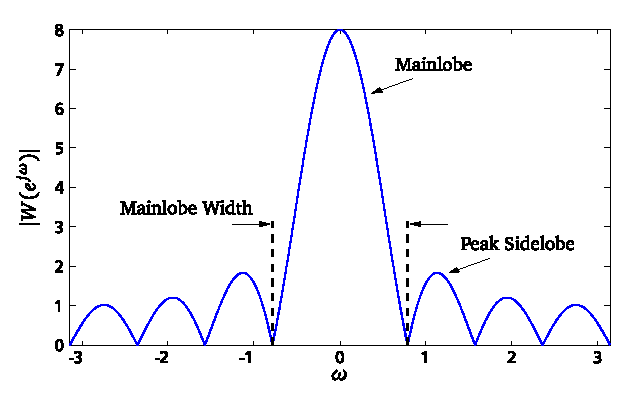
\includegraphics[width=\textwidth]{figures/main_side_lobes.pdf}

\subsubsection{Peak approxomation error (PAE)}
\begin{equation}
 PAE =\gamma \cdot \max\limits_{\omega \in \mathbb{R}} \left|H_d\freq - H\freq\right|
\end{equation}
The PAE is also directly related to the maximum allowable specification tolerance.
With $\omega_c$ as the discontinuity of $H_d\freq$: 
\begin{equation}
\Delta H_d\left(e^{j\omega_c}\right) \cdot \gamma \leq \min(\alpha_1,\alpha_2)
\end{equation}


\subsubsection{Commonly used Windows}
\begin{subequations}
\begin{align}
\text{Rectangular} \notag \\
w(n) &= \begin{cases}
1 &,0\leq n \leq N-1\\
0		&\text{, otherwise}
\end{cases}\\
\text{Barlett} \notag \\
w(n) &= \begin{cases}
\frac{2n}{N-1} &,0\leq n \leq \frac{N-1}{2}\\
2-\frac{2n}{N-1}		&,\frac{N-1}{2}\leq n\leq N-1
\end{cases}\\
\text{Hanning} \notag \\
w(n)& = \frac{1}{2}\left[1-\cos\left(\frac{2\pi n}{N-1}\right)\right] \quad 0\leq n \leq N-1\\
\text{Hamming} \notag \\
w(n)& = 0.54-0.46\cos\left(\frac{2\pi n}{N-1}\right) \quad 0\leq n \leq N-1 \\
\text{Blackman} \notag \\
w(n)& = 0.42-0.5\cos\left(\frac{2\pi n}{N-1}\right)+0.08\cos\left(\frac{4\pi n}{N-1}\right) \quad 0\leq n \leq N-1
\end{align}
\end{subequations}
These windows have different Properties: \\
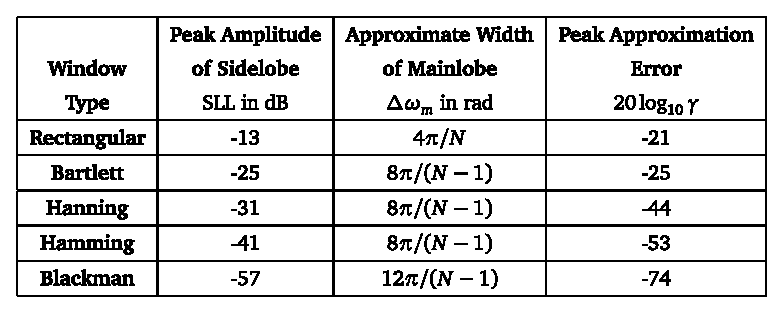
\includegraphics[width=\textwidth]{figures/window_props.pdf}


\subsection{Kaiser Window Filter Design}
The Kaiser window function adapts to the specifications. Let $\alpha = \frac{N-1}{2}$ and $I_0$ be the zeroth
order modified Bessel function of the first kind, while $\beta$ is a shape parameter:
\begin{equation}
w(n)=\begin{cases}
\frac{I_0\left\{\beta\left[1-\left(\frac{n-\alpha}{\alpha}\right)^2\right]^{\frac{1}{2}}\right\}}{I_0(\beta)} &,0\leq n\leq N-1\\
0 &,\text{otherwise}
\end{cases}
\end{equation}

\subsubsection{Design a filter with Kaiser window}
Assuming the transition region is $\Delta\omega = \omega_s-\omega_p$. With $A = -20\log_{10}\min(\alpha_1,\alpha_2)$
\begin{equation}
\beta = \begin{cases}
0.1102(A-8.7) &A>50 \\
0.5842(A-21)^{0.4}+0.07866(A-21) &21\leq A \leq 50 \\
0 &A<21
\end{cases}
\end{equation}
and
\begin{equation}
N=\left[\frac{A-8}{2.285\Delta\omega}+1\right]
\end{equation}
\subsubsection{Integrated Square Error}
To optimize a windowed filter, one has to attempt to minimize the integrated squared error
\begin{equation}
\epsilon^2=\frac{1}{2\pi}\int\limits_{-\pi}^{\pi}\left|H_d\freq - H\freq\right|^2 d\omega
\end{equation}

\subsection{Optimal Filter Design}
Optimal filter design does not use the integrated square error but instead the maximum error, which occurs at the discontinuities of $H_d\freq$.
This error gets distributed equally across the frequency band.
Please use the script pages 33-36 for information about optimal filter design.

\section{Infinite Impulse Response (IIR) filter}
IIR filters are systems, which follow the following restrictions:\\
$h(n)$ is
  \begin{itemize}
  	\item real
  	\item causal
  	\item satifies stability
  \end{itemize}
$h(n)$ possesses a rational z-transform with $a_0=1$, i.e.
\begin{equation}
  	H(z)=\frac{\sum\limits_{k=0}^{N-1} b_k z^{-k}}{1-\sum\limits_{k=0}^{N-1} a_k z^{-k}}
\end{equation}
  
 
\subsection{Properties of IIR filters}
\begin{itemize}
  \item {\bf Stability}\\ All poles of $H(z)$ must lie inside the unit disk
  \item {\bf Linear Phase}\\ IIR filters do not have linear phase. Only the magnitude response is specified.
\end{itemize}

\subsection{IIR filter design from an analog or continuous-time filter (Impulse Invariance Method)}
Steps to design:
\begin{itemize}
  \item {\bf Step 1}: Specification of the digital filter
  \item {\bf Step 2}: Translation to a continuous-time filter specification
  \item {\bf Step 3}: Determination of the continuous-time filter system function $H_c(s)$
  \item {\bf Step 4}: Transformation of $H_c(s)$ to a digital filter system function $H(z)$
\end{itemize}
\subsubsection{Step 1}
Filter parameters like $\alpha_1,\alpha_2,\omega_p,\omega_s$ and $T_d$ have to be set.
\subsubsection{Step 2}
If a Filter $H_c(\Omega)$ is given, applying the relation $\Omega=\omega/T_d$ leads to the continuous-time filter specifications, where $T_d$ 
is the design sampling interval. Then the filter has to be checked to fulfil the Specifications given in Step 1

\subsubsection{Step 4}
Steps for the transformation of $H_c(s)$ to $H(z)$
\begin{enumerate}
  \item From $H_c(s)$ and $H_c(j\Omega)$, we determine $h_c(t)$
  \item Optain the digital sequence by $h(n)=T_d\cdot h_c(nT_d)$ where $T_d$ is the design sampling interval
  \item $H(z)$ is obtained from $h(n)$
\end{enumerate}
\subsection{The Butterworth filter}
With $\Omega_c$ being the $3\text{dB}$ cut-off frequency
\begin{equation}
\left|H(j\Omega)\right|^2=\frac{1}{1+\left(\frac{\Omega}{\Omega_c}\right)^{2N}}
\end{equation}
With the conditions $\left|H(j\Omega)\right|\geq 1-\alpha_1$ for $0\leq|\Omega|\leq\Omega_p$ and $\left|H(j\Omega)\right| \leq \alpha_2$ for $\Omega_s\leq|\Omega|$ 
\begin{subequations}
\begin{align}
N& \geq \frac{\log\left(\frac{1}{(1-\alpha_1)^2}-1\right)-\log\left(\frac{1}{\alpha_2^2}-1\right)}{2(\log\left(\Omega_P\right)-\log\left(\Omega_S\right))}\\
\Omega_c&=\frac{\Omega_S}{\sqrt[2N]{\frac{1}{\alpha_2^2}-1}}\\
\Omega_c &= \frac{\Omega_P}{\sqrt[2N]{\frac{1}{(1-\alpha_1)^2}-1}}
\end{align}

\end{subequations}
\subsection{Bilinear Transformation}
The bilinear transformation is used to map the imaginary axis of the $s$-plane to the unit circle.
Now let
\begin{subequations}
\begin{equation}
s=\frac{2}{T_d}\left[\frac{1-z^{-1}}{1+z^{-1}}\right]
\end{equation}
which leads to
\begin{equation}
H(z) = H_c\left[\frac{2}{T_d}\left(\frac{1-z^{-1}}{1+z^{-1}}\right)\right]
\end{equation}
with $z=e^{j\omega}$:
\begin{equation}
s=\frac{2}{T_d}\left[\frac{1-e^{-j\omega}}{1+e^{-j\omega}}\right]=j\frac{2}{T_d}\tan(\omega/2)
\end{equation}
with $s=\sigma + j\Omega$ follows:
\begin{equation}
\Omega=\frac{2}{T_d}\tan(\omega/2) \text{ and } \sigma = 0
\end{equation}
\end{subequations}

\subsubsection{Remarks on the bilinear transformation}
\begin{itemize}
  \item The frequency deformation $\Omega=\frac{2}{T_d}\tan(\omega/2)$ comes to a deviation in the detailed shape of $H_c(j\Omega)$
  \item The delay time is also modified: $\tau_d=\tau_c\left\{1+\frac{\omega_c T_d}{2}\right\}$
  \item The bilinear transformation has no aliasing problems.
  \item This transformation is the most used in practise
\end{itemize}

\subsubsection{Conversion from continuous-time to system function}
Let $\Omega_c$ be the cutoff-frequency and $s_k=\Omega_c \cdot e^{j\frac{\pi}{2N}(2k+N+1)}$ for $k=0,\ldots,N-1$ be the poles of the function. Take those who are on the left half plane and:
\begin{equation}
H(s)=\prod\limits_{k=0}^{N-1} \frac{\Omega_C^N}{s-s_k}
\end{equation}  
\subsection{Implementation of IIR Filters}
The output of the filter can be described as
\begin{equation}
y(n) = \sum\limits_{k=1}^{M}a_k y(n-k)+\sum\limits_{r=0}^{N-1}b_r x(n-r)
\end{equation}
\subsubsection{Direct Form I}
A Signal flow graph can be seen at Figure 5.8 on page 47 in the DSP script.
\begin{equation}
H(z)=H_2(z)H_1(z)=\left(\frac{1}{\sum\limits_{k=1}^{M}a_k z^{-k}}\right)\left(\sum\limits_{r=0}^{N-1}b_rz^{-r}\right)
\end{equation}
\subsubsection{Direct Form II}
The direct form II can change the order of $H_1(z)$ and $H_2(z)$. A Signal flow graph can be seen at Figure 5.9 on page 48 in the DSP script.
\begin{equation}
H_1(z)H_2(z)=H(z)=H_2(z)H_1(z)
\end{equation}
\subsubsection{Cascade Form}
A Signal flow graph can be seen at Figure 5.10 on page 48 in the DSP script.
\begin{subequations}
\begin{align}
H(z)&=\frac{\sum\limits_{r=0}^{N-1}b_rz^{-r}}{1-\sum\limits_{k=1}^{M}a_k z^{-k}}=A\prod\limits_k H_k(z)\\
\text{with} \notag\\
H_k(z)&=\frac{1+\beta_{1k}z^{-1}+\beta_{2k}z^{-2}}{1-\alpha_{1k}z^{-1}-\alpha_{2k}z^{-2}}
\end{align}
\end{subequations}

\section {Filter Specficaion}
Non-ideal Filters have one or more pass-bands($\omega_p$), 
transition-bands(between $\omega_p$ and $\omega_s$) and stop-bands($\omega_s$). 
For the pass- and the stop- band, a tolerance
$\alpha_i$ has to be specified. Therefore a low-pass filter would have the following specification:
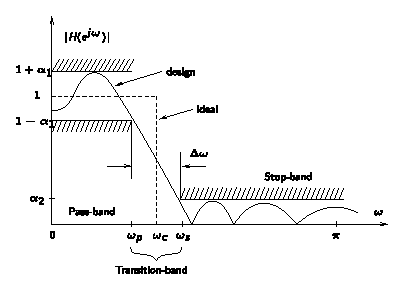
\includegraphics[width=\textwidth]{figures/filter_spec.pdf}

\subsection{Ripple and Attenuation calculation}
Given the pass-band attenuation   $\text{ATT}_P$ and the stop-band attenuation $\text{ATT}_S$ of an IIR filter
\begin{subequations}
\begin{align}
\alpha_1&=1-10^{-\text{ATT}_P/20}\\
\alpha_2&=10^{-\text{ATT}_S/20}
\end{align}
Given the pass-band ripple $\text{R}_P$ and the stop-band ripple $\text{R}_S$ of a FIR Filter 
\begin{align}
\alpha_1&=10^{\text{R}_P/20}-1 \\
\alpha_2&=10^{-\text{R}_S/20}
\end{align}
\end{subequations}
\chapter{Random Variables and Stochastic Processes}
This is a revision of the Stochastic Signals and Systems course, which has an own Formulary which can be found at:
\url{https://github.com/Tyde/stosigsysfs/blob/master/document.pdf?raw=true}
\chapter{The Finite Fourier Transform}
\section{Definition}
Let $x(0),\ldots,x(N-1)$ be realisiations of a stationary random process $X(n),n=0,1,2,\ldots,N-1$
\begin{equation}
X_N\freq = \sum\limits_{n=0}^{N-1}X(n)e^{-j\omega n}, \quad -\infty < \omega \infty 
\end{equation} 
and inverse:
\begin{equation}
X(n)=\frac{1}{2\pi}\int\limits_{-\pi}^{\pi}X_N\freq e^{j\omega n}d\omega, \quad n=0,1,\ldots,N-1
\end{equation}

\subsection{Properties}
\begin{itemize}
  \item {\bf Periodicity} $X_N\left(e^{j(\omega +k2\pi}\right)=X_N\freq\quad\forall k \in \mathbb{N}$
  \item {\bf Symmetry} $X_N\left(e^{-j\omega}\right)=X_N\freq^{*}\quad \forall X(n) \in \mathbb{R}$
  \item {\bf Linearity} $\mathcal{F}\{aX(n)+bY(n)\} = aX_N\freq + bY_N\freq$
\end{itemize}
\section{Discrete Finite Fourier Transform}
With $\omega_k=2\pi k/N, k=0,\ldots,N-1$
\begin{equation}
X_N(e^{j\frac{2\pi k}{N}})=\sum\limits_{n=0}^{N-1}X(n)e^{-j2\pi kn/N} \quad,k=0,1,\ldots,N-1
\end{equation}

\section{Statistical Properties}
\subsection{White Gaussian Process}
Let $X(0),\ldots,X(N-1)$ be real valued random variables with $X(n)\sim\mathcal{N}(0,1)$ and $N=2^r$ with $r \in \mathbb{N}$
Then:
\begin{subequations}
\begin{align}
\mathfrak{Re}\left\{X_N(e^{j2\pi k/N})\right\} = \sum\limits_{n=0}^{N-1} X(N)\cos(2\pi kn/N)\\
\mathfrak{Im}\left\{X_N(e^{j2\pi k/N})\right\} = -\sum\limits_{n=0}^{N-1} X(N)\sin(2\pi kn/N)
\end{align}
The Mean and Variance can be determined to:
\begin{align}
\begin{bmatrix}
\mathfrak{Re}\left\{X_N(e^{j2\pi k/N})\right\}\\
\mathfrak{Im}\left\{X_N(e^{j2\pi k/N})\right\}\\
\end{bmatrix} \sim \mathcal{N}\left( \begin{bmatrix}0\\0\end{bmatrix}, \frac{N}{2}
\begin{bmatrix}1&0\\0&1\end{bmatrix}\right)
\end{align}
\end{subequations}

\subsection{Real Stationary Random Process}
If the process has an arbitray $\mu_x,c_{XX}(\kappa)$ and $C_{XX}\freq$ for $N\rightarrow\infty$ the asymptotic distribution is:
\begin{subequations}
\begin{equation}
\begin{bmatrix}
\mathfrak{Re}\left\{X_N\freq\right\}\\
\mathfrak{Im}\left\{X_N\freq\right\}\\
\end{bmatrix} \sim \mathcal{N}\left( \begin{bmatrix}0\\0\end{bmatrix}, \frac{N}{2}C_{XX}\freq
\begin{bmatrix}1&0\\0&1\end{bmatrix}\right) \quad \omega \in (0,\pi)
\end{equation}
For $\omega = 0$ and $\omega = \pi$ The Finite Fourier Transform is purely real:
\begin{equation}
\mathfrak{Re}\left\{X_N\freq\right\} \sim \mathcal{N} \left(N\mu_x\delta(\omega),NC_{XX}\freq\right)
\end{equation} 
For fixed frequencies $0 \leq \omega_{(1)} < \ldots < \omega_{(M)} \leq \pi$ the random variables
$X_N(e^{j\omega_{(1)}}),X_N(e^{j\omega_{(2)}}),\ldots,X_N(e^{j\omega_{(M)}})$ are asomptotically for $N\rightarrow\infty$
{\bf indepently distributed}
\end{subequations}
\section{Segmentation of the Finite Fourier Transform}
Division of random process $X(n), n=0,\ldots,N-1$ into L segments of length M with $N=ML$ will yield a finite fourier transform
for each segment $l$ which has the same asymptotic distribution as for the non-segmented process 
\begin{equation}
X_M(e^{j\omega},l)=\sum\limits_{n=0}^{M-1}X(n-(l-1)M)e^{-j\omega n}, \quad l=1,\ldots,L
\end{equation}
The random variables $X_M(e^{j\omega},l)$ arre for $l=1,\ldots,L$ asymptotically as $N\rightarrow\infty$ indepently distributed

\section{Windowing of the process}
Let $w(n)=0$ for $n=0,\ldots,N-1$ be a window that is applied to the random process.
\begin{equation}
X_{n,\omega} \freq=\sum\limits_{n=0}^{N-1} w(n)X(n)e^{-j\omega n}
\end{equation}
The window has the effect that the variance is multiplied by the factor $\sum_{n=0}^{N-1}w(n)^2$
and the mean at $\omega=0$ is multiplied by the factor $\sum_{n=0}^{N-1} w(n)$

\subsection{Power of the windowed process}
The average power of $X(n)$ is defined by
\begin{equation}
P_{XX}=\lim\limits_{N\rightarrow\infty}\frac{1}{N}\sum\limits_{n=0}^{N-1}\E\left[X(n)^2\right] =
\lim\limits_{N\rightarrow\infty}\frac{1}{2\pi}\int\limits_{-\pi}^{\pi}\frac{1}{N}\E\left[\left|X_N\freq\right|^2\right] d\omega
\end{equation}

\chapter{Digital Spectral Analysis}
\section{Consitency and Mean Square Error in terms of bias and variance}
The MSE can be rewirtten as follows:
\begin{equation}
\text{MSE}(\hat{\mu}_X)=\Var \left[\hat{\mu}_X\right] + \text{bias}(\hat{\mu}_X)^2
\end{equation}
The Estimator $\hat{\mu}_X$ is called consisten if:
\begin{equation}
\lim\limits_{N\rightarrow\infty} \text{MSE}(\hat{\mu}_X) = 0
\end{equation}
\section{Mean Estimation}
The mean of $X(0),\ldots ,X(N-1)$ which are ech distributed as $\mathcal{N}(\mu_X,\sigma_X^2)$, can be estimated by:
\begin{equation}
\hat{{\mu}}_x=\frac{1}{n}\sum\limits_{n=0}^{N-1}X(n)
\end{equation}

\section{The Periodogram}
A candiate estimator for $C_{XX}\freq$ is the periodogram:
\begin{equation}
I_{XX}^{N}\freq = \frac{1}{N}\left|X_N\freq\right|^2 = \frac{1}{N}\left|\sum\limits_{n=0}^{N-1} X(n) e^{-j\omega n}\right|^2
\end{equation}
\subsection{Distribution of the Periodogram}
The periodogram for data values $X(N)$ is indepently distributed as:
\begin{equation}
I_{XX}^{N} \sim \begin{cases}
\frac{C_{XX}\freq}{2}\chi_2^2 &,\omega \neq \pi k \\
C_{XX}\freq\chi_1^2 &,\omega = \pi k \\
\end{cases}
\end{equation}

\subsection{Mean of the Periodogram}
With the use of (\ref{geomconv})
\begin{subequations}
\begin{align}
\E\left[I_{XX}^{N}\freq\right] &= \frac{\left|\Delta^N\freq\right|}{N} \circledast C_{XX}\freq 
+\frac{\left|\Delta^N\freq\right|}{N} \cdot \left|\mu_x\right|^2 \\
\text{where} \notag \\
\Delta^N\freq &= \sum\limits_{n=0}^{N-1}e^{-j\omega n} = e ^{-j \omega \frac{N-1}{2}} \cdot \frac{\sin(\frac{\omega N}{2})}{\sin(\frac{\omega}{2})}
\end{align}

\end{subequations}
Thus for a zero mean stationary process $X(n),\E\left[I_{XX}^{N}\freq\right]$ for $N\rightarrow\infty$
\begin{subequations}
\begin{align}
\lim\limits_{N\rightarrow\infty} \E\left[I_{XX}^{N}\right] &= C_{XX}\freq \quad \omega \neq 2k\pi \\
\lim\limits_{N\rightarrow\infty} \E\left[I_{X-\mu_x,X-\mu_x}^{N}\right] &= C_{XX}\freq \quad \forall\omega
\end{align}
\end{subequations}

\subsection{Variance of the Periodogram}
Let $X(n)$ be a real white Gaussian Process with $\sigma^2$ and $\omega,\lambda \neq 0$
\begin{equation}
\Var\left[I_{XX}\freq\right] \approx C_{XX}\freq^2 \cdot \frac{1}{N^2}(|\Delta^N(e^{j2\omega})|^2+N^2)
\end{equation}
Therefore the Periodogram is not a consistent estimator

\subsection{Averaging Periodograms (Barlett's method)}
To improve the consistency of the Periodogram, it is 
possible to average the estimates of multiple independent measurements. With $X_l(n)=X(n+(l-1)\cdot M)$ and $n=0,\ldots,M-1$
\begin{equation}
I_{XX}^M(e^{j\omega},l)=\frac{1}{M}\left|\sum\limits_{n=0}^{M-1} X_l(n) e^{-j\omega n}\right|^2 \quad = 1,\ldots,L
\end{equation}
And estimate with:
\begin{equation}
\hat{C}_{XX}^B\freq = \frac{1}{L}\sum\limits_{l=1}^{L} I_{XX}^M (e^{j\omega},l)
\end{equation}
{\bf The variance of Barlett's estimator decreases when L increases}

\subsubsection{Mean and Variance of Barlett's method}
\begin{subequations}
\begin{align}
\E\left[\hat{C}_{XX}^B\right]&=\frac{1}{L}\sum\limits_{l=1}^L \E\left[I_{XX}^M(e^{j\omega},l)\right] \approx \E \left[I_{XX}^M\freq\right]\\
\Var\left[\hat{C}_{XX}^B\right]&=\frac{1}{L^2}\sum\limits_{l=1}^L \Var\left[I_{XX}^M(e^{j\omega},l)\right] \approx \frac{1}{L}\Var \left[I_{XX}^M\freq\right]
\end{align}
\end{subequations}
\subsection{Welch's method}
Welch's method is similar to Barlett's method but the data segments are multiplied by a window $w_M(n)$ of length
$M$ and the segmens may overlap. With $X_l(n)=X(n+(l-1)\cdot D)$
\begin{subequations}
\begin{align}
\hat{C}_{XX}^W\freq &= \frac{1}{L}\sum\limits_{l=1}^L I_{WX,WX}^M (e^{j\omega},l) \\
\text{and} \notag \\
I_{WX,WX}^M(e^{j\omega},l)&= \frac{1}{MA}\left|\sum\limits_{n=0}^{M-1} w_M(n) \cdot X_l(n) e^ {-j\omega n}\right|^2
\end{align}
Where $A$ is a factor to ge an asymptotic unbiased estimation, which can be found using Parseval's theorem:
\begin{equation}
\frac{1}{2\pi}\int\limits_{-\pi}^{\pi} \left| W_M(e^{j\lambda}) \right|^2 d\lambda = \sum\limits_{n=0}^{M-1}\left|w_M(n)\right|^2 =MA
\end{equation}
\end{subequations}

\subsubsection{Mean of Welch's Estimator}
\begin{subequations}
\begin{align}
\E\left[\hat{C}_{XX}^W\freq\right]&=\frac{1}{L}\sum\limits_{l=1}^L
\E\left[I_{WX,WX}^M(e^{j\omega},l)\right] \approx
\E\left[I_{WX,WX}^M(e^{j\omega})\right] \\
\text{with} \notag \\
\E\left[I_{WX,WX}^M\freq\right] &\approx C_{XX}\freq \quad \omega \neq 0
\end{align}
\end{subequations}
\subsection{Smoothing the Periodogram}
With $\omega_k\neq\omega_l$, thus $X_N(e^{j\omega_k})$ and $X_N(e^{j\omega_l})$ are asymptotically independent and 
$I_{XX}^N(e^{j\omega_k})$ and $I_{XX}^N(e^{j\omega_l})$ are also independent:
\begin{equation}
\hat{C}_{XX}^S\freq = \frac{1}{2m+1}\sum\limits_{k=-m}^m I_{XX}^N
\left(e^{j2\pi(k(\omega)+k)/N}\right)
\end{equation}
\subsubsection{Variance of the smoothed Periodogram}
\begin{equation}
\lim\limits_{N\rightarrow\infty} \Var\left[\hat{C}_{XX}^S\freq\right] = \frac{1}{2m+1} C_{XX}\freq^2
\end{equation}


\subsection{Generall Class of Spectral Estimates}
Wit $A=\frac{1}{2m+1}\sum_{k=-m}^m W_k$ a generall class of estimators can be defined analogusly to the smoothed periodogram
\begin{equation}
\hat{C}_{XX}^{SW}\freq = \frac{1}{(2m+1)A}\sum\limits_{k=-m}^m W_kI_{XX}^N(e^{j2\pi(k(\omega)+k)/N})
\end{equation}

\section{The Log-Spectrum}
Estimating $10\log C_{XX}\freq$ from $10\log \hat{C}_{XX}\freq$ instead of the spectrum
\section{The Blackman-Tuckey Method}
This Mehthod estimates the sample covariance function and windows it with $w_{2M-1}(\kappa)$
\begin{subequations}
\begin{align}
w_{2M-1}(\kappa) &= \begin{cases}
w_{2M-1}(-\kappa) &,\text{for } |\kappa|\leq M-1 ,\text{with } M\ll N\\
0 &,\text{otherwise}\end{cases}\\
\hat{C}_{XX}^{BT}\freq &= \sum\limits_{\kappa=-M+1}^{M-1} \hat{c}_{XX}(\kappa )\cdot w_{2M-1}(\kappa)\cdot e^{-j\omega\kappa}\\
\text{This is the same as} \notag\\
\hat{C}_{XX}^{BT}\freq &= \frac{1}{2\pi} \int\limits_{-\pi}^\pi I_{X-\bar{X},X-\bar{X}}^N(e^{j\lambda})\cdot W_{2M-1}\left(e^{j(\omega-\lambda}\right)d\lambda\\
\text{This has the following}&\text{ constraint for the window:} \notag\\
W_{2M-1}\freq &\geq 0 \quad\quad \forall \omega
\end{align}

The Blackman-Tukey estimator is unbiased for $N\rightarrow\infty$ and its variance tends to zero if the window function has finite energy.
The Variance of the Blackman-Tuckey Method is defined by:
\begin{equation}
\Var\left[\hat{C}_{XX}^{BT}\right]\approx C_{XX}\freq^2 \frac{1}{N} \sum\limits_{\kappa=-M+1}^{M-1} w_{2M-1}(\kappa)^2
\end{equation}

\end{subequations}
\section{Cross-Spectrum Estimation}
\subsection{The Cross-Periodogram}
For $X(0),\ldots ,X(N-1),Y(0),\ldots,Y(N-1)$ the objective is to estimate the cross-spectrum $C_{YX}\freq$ for $-\pi <\omega <\pi$
\begin{equation}
I_{YX}^N\freq=\frac{1}{N}Y_N\freq X_N\freq^{*}
\end{equation}
This has the bias $C_{YX}\freq$ and the variance $C_{YY}\freq C_{XX}\freq$
\subsection{Segmented Cross-Periodogram}
For different Segments $l=1,\ldots,L$ with length $M$
\begin{subequations}
\begin{align}
\hat{C}_{YX}^B\freq &= \frac{1}{L}\sum\limits_{l=1}^L \frac{1}{M} Y_M(e^{j\omega},l)X_M(e^{j\omega},l)^{*} \\
\text{with}\notag \\
Y_N(e^{j\omega},l) &= \sum\limits_{n=0}^{M-1} Y(n-(l-1)M)e^{-j\omega n}\\
X_N(e^{j\omega},l) &= \sum\limits_{n=0}^{M-1} X(n-(l-1)M)e^{-j\omega n}
\end{align}
Now for $N\rightarrow\infty$ the bias is $C_{YX}\freq$ and the variace is $\frac{1}{L}C_{YY}\freq C_{XX}\freq$
\end{subequations}

\chapter{Parametric Spectrum Estimation}
\section{Auto-regressive (AR) Processes}
With 
\begin{equation}
C_{XX}\freq = \frac{\sigma_Z^2}{\left|1+\sum_{k=1}^p a_k e^{-j\omega k} \right|^2}
\end{equation}
The objective is to estimate the parameter $a_1,\ldots,a_p$ which will be used to estimate the spectrum $C_{XX}\freq$
\subsection{Yule-Walker Equations}
\begin{equation}
c_{XX}(l)+ \sum\limits_{k=1}^p a_kc_{xx}(l-k)=\begin{cases}
\sigma_Z^2 &,l=0\\
0 &,l=1,\ldots,p
\end{cases}
\end{equation}
Using $\hat{c}_{XX}(0),\ldots,\hat{c}_{XX}(p)$ leads to a unique solution for $a_1,\ldots,a_p$

\subsection{extended Yule-Walker equations}
$Z(n)$ and $V(n)$ are uncorrelated white noise processes with variances $\sigma^2_Z$ and $\sigma_V^2$. With the
differencee equation of the system $Y(n)+aY(n-1)=Z(n)+V(n)+aV(n-1)$
\begin{equation}
c_{YY}(l)+\sum\limits_{k=1}^p a_kc_{YY}(l-k) =\begin{cases}
\sigma_Z^2+\sigma_V^2 &,l=0 \\
a_l\sigma_V^2 &,l=1,\ldots,p\\
0 &,l>p 
\end{cases}
\end{equation}

\section{Moving Average (MA) Process}
Consider a transversal filter $h(n)$ with input real-valued $Z(n)$ and real-valued output $X(n)$
\begin{equation}
X(n)=\sum\limits_{k=0}^q h(k)Z(n-k)
\end{equation} 
If $Z(n)$ is a white noise process, $X(n)$ is a {\bf Moving average (MA) process} with
\begin{equation}
C_{XX}=\left|H\freq\right|^2C_{ZZ}\freq =\left|H\freq\right|^2\sigma_Z^2 
\end{equation}
With $b(m)=\sigma_Z h(m)$ and $m=0,\ldots,q$ and $h(0)=1$ we get
\begin{align}
c_{XX}(l)&=\sum\limits_{m=0}^{q-|l|} b(m)b(m+|l|) \quad \text{for } 0\leq |l| \leq q\\
\text{and}\\
C_{XX} &= B\freq B(e^{-j\omega})
\end{align}
\subsection{Solving} \label{solv}
\begin{enumerate}
  \item substitute $e^{j\omega}$
  \item Calculate $P(z)=z^qC_{XX}(z)$
  \item Assign all roots $z_i$ of $P(z)$ inside the unit circle to $B(z)$ \\
  		$B(z)=b(0)\prod_{i=1}^q(1-z_iz^{-1})$ with $b(0)>0$ and $|z_i|\leq 1$
  \item Calculate $h(m)=b(m)/b(0)$ for $m=1,\ldots,q$\\ 
		With $b(0)^2=\sigma_Z^2=\frac{c_{XX}(0)}{1+\sum_{m=1}^q h(m)^2}$ and replacing $c_{XX}(l)$ with $\hat{c}_{XX}(l)$ 
\end{enumerate}
The Spectrum can be obtained by the relationship
\begin{equation}
\hat{C}_{XX}\freq = \left|\sum\limits_{n=0}^q \hat{b}(n)e^{-j\omega n} \right|^2
\end{equation}

\section{Auto-regressive Moving Average (ARMA) Process}
The difference equation of an ARMA process, called $ARMA(p,q)$, is given by
\begin{equation}
X(n)+\sum\limits_{k=1}^p a_kX(n-k) = Z(n)+\sum\limits_{k=1}^q b_k Z(n-k)
\end{equation}
The modified Yule-Walker equations can be found:
\begin{equation}
c_{XX}(l)+\sum\limits_{k=1}^p a_k c_{XX}(l-k) = \begin{cases}
\sigma_Z^2\sum_{k=l}^q b_kh(k-l) &,l=0,\ldots,q\\
0&,l>q
\end{cases}
\end{equation}
To solve for $a_1,\ldots,a_p$, the equations can be employed with $l=q+1,\ldots,q+p$. Then to determine $b_1,\ldots,b_q$ , $l=1,\ldots,q$ are used with (\ref{solv})

\section{Model order selection}
\subsection{Akaine's Information Criterion (AIC)}
\begin{equation}
\text{AIC}(m)=\log \hat{\sigma}_{Z,m}^2 + m\frac{2}{N} \quad m=1,\ldots,M
\end{equation}
\subsection{Minimum Description Length (MDL)}
\begin{equation}
\text{MDL}(m)=\log \hat{\sigma}_{Z,m}^2 + m\frac{\log N}{N} \quad m=1,\ldots,M
\end{equation}
\chapter{Miscellaneous}
\section{Useful mathematical equations}
\subsection{Geometric series}
\begin{equation}
\sum\limits_{n=0}^{N-1} q^n = \frac{1-q^N}{1-q} \quad \text{for} \quad|q|<1
\end{equation} 



\subsection{Conversion from Geometric series to trigonometric fraction} \label{geomconv}
Let $\frac{1-q^{N}}{1-q}$ be with $q = e^{-j\omega}$
\begin{equation}
\frac{1-e^{-jN\omega}}{1-e^{-j\omega}} = e^{-j\omega \frac{N-1}{2}}\frac{\sin\left(\frac{N}{2}\omega\right)}{\sin\left(\frac{\omega}{2}\right)}
\end{equation}

\subsection{Modulation Theorem}
Let $\mathcal{F}\left\{f(x)\right\}=F\freq$ be the fourier transform, then:
\begin{equation}
\mathcal{F}\left\{\cos(2\pi k_0 x)f(x)\right\} = \frac{1}{2}\left[F(k-k_0)+F(k+k_0)\right]
\end{equation}
\end{document}

